\documentclass{article}

\usepackage[spanish,es-tabla]{babel}
\usepackage[utf8]{inputenc}
\usepackage{color}
\usepackage{listings}
\usepackage{xcolor}
\usepackage{graphicx}
\usepackage{caption}


\definecolor{dkgreen}{rgb}{0,0.6,0}
\definecolor{gray}{rgb}{0.5,0.5,0.5}
\definecolor{darkred}{rgb}{0.55, 0.0, 0.0}
\definecolor{darkgray}{rgb}{0.88, 0.88, 0.88}

\graphicspath{ {./Imagenes/} }
\DeclareGraphicsExtensions {.pdf,.png,.jpg}



\lstset{
  aboveskip=3mm,
  belowskip=3mm,
  showstringspaces=false,
  columns=flexible,
  basicstyle={\small\ttfamily},
  numbers=none,
  numberstyle=\tiny\color{gray},
  keywordstyle=\color{blue},
  commentstyle=\color{dkgreen},
  stringstyle=\color{darkred},
  breaklines=true,
  breakatwhitespace=true,
  tabsize=3,
  backgroundcolor=\color{darkgray},
}


\title{Instalacion de Django}
\author{Enrique García González}




\begin{document}


\maketitle

Este documento se trata una guia de como realizar la instalación de Django y los elementos
necesarios para el correcto funcionamiento de la aplicación web, asi como un pequeño 
manual para iniciarse con Django

\newpage

\tableofcontents

\newpage

\section{Instalacion y puesta en marcha}

En primer lugar, para instalar Django en una distribución ubuntu o debian necesitamos contar
con una instalación previa de Python. En este caso suponiendo que partimos de una instalacion
correcta de python 3.5 debemos instalar las siguientes librerias con pip.


\lstset{
  language=Bash,
}
\begin{lstlisting}
pip3 install django
pip3 install gunicorn
pip3 install psycopg2
\end{lstlisting}

Para crear un proyecto de django debemos ejecutar el siguiente comando dentro de la carpeta
donde queremos que se almacene

\begin{lstlisting}
django-admin startproject <nombre proyecto>
\end{lstlisting}

El cual nos genera la estructura basica del proyecto. Ahora entramos en esta carpeta y comprobamos 
que tenemos un directorio con el mismo nombre del proyecto y un archivo llamado manage.py. En este
directorio creamos una carpeta llamada templates, que sera la encargada de almacenar el código html
del proyecto.

\begin{lstlisting}
mkdir templates
\end{lstlisting}

Después entramos en el directorio que tiene el mismo nombre que el proyecto el archivo views.py

\begin{lstlisting}
cd <nombre proyecto
touch views.py
\end{lstlisting}

Al hacer esto nos tiene que quedar una estructura parecida a la siguiente

\begin{center}
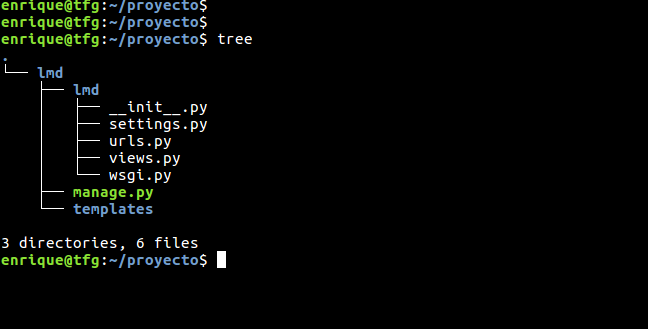
\includegraphics[scale=0.5]{img}
\captionof{figure}{Estructura proyecto}\label{fig:Estructura Proyecto}
\end{center}



\section{Organización de un proyecto en Django}

Este punto esta creado para orientar un poco sobre la organización de un proyecto
en Django a aquellos usuarios que no lo han utilizado nunca.

Django sigue una estructura de MOdelo-ista-Controlador, aunque no usa su propia lógica en
la implementacion, ya que la capa Controlador es manejada por el framework. Por esto las partes más interesantes son:

\begin{description}
	\item[Model:] Es la capa de acceso a datos. COntiene todo sobre los datos: acceso, 
	validación, relaciones entre ellos,etc.
	\item[Template:] Capa de representación. Contiene la información sobre como se tienen que 
	mostrar las cosas en la página Web
	\item[View:] Esta capa que contiene la lógica de acceso a la capa Model y se la ofrece
	al Template apropiado. Es como un puente entre las dos capas anteriores.
\end{description}



\section{Templates}

Un template de Django es una cadena de texto que se utiliza para separar la representación
de la página de los datos. Contienen también algunas reglas lógicas para regular
que partes de la página se tienen que mostar y se encarga de generar el código html. La
forma más comoda y ordenada de hacerlo es crear para cada página un fichero html dentro
de la carpeta templates. Para poder utilizar este método tenemos que modificar el archivo
settings.py (podemos ver donde se encuentra en la figura 1). Buscamos la parte
correspondiente a los templates, que es de la siguiente forma:


\lstset{
  language=Python,
}
\begin{lstlisting}
TEMPLATES = [
    {
        'BACKEND': 'django.template.backends.django.DjangoTemplates',
        'DIRS': [],
        'APP_DIRS': True,
        'OPTIONS': {
            'context_processors': [
                'django.template.context_processors.debug',
                'django.template.context_processors.request',
                'django.contrib.auth.context_processors.auth',
                'django.contrib.messages.context_processors.messages',
            ],
        },
    },
]
\end{lstlisting}

Modificamos la linea DIRS para que quede de la siguiente forma

\begin{lstlisting}
'DIRS': [os.path.join(BASE_DIR, 'templates')],
\end{lstlisting}

De esta forma ya podemos utilizar la carpeta templates, creada en el apartado 1 para
almacenar todos nuestros templates.

\hspace{1cm}

Para más información sobre los templates en django:

\hspace{1cm}

http://djangobook.com/django-templates/

http://djangobook.com/basic-template-tags-filters/

http://djangobook.com/templates-in-views/

http://djangobook.com/advanced-templates/


\section{Templates}

Si queremos que nuestro servidor web sea accesile para otras máquinas, primero debemos
modificar el archivo settngs.py. Buscamos las líneas donde aparecen DEBUG y ALLOWED\_HOST y 
las dejamos de la siguiente manera


\lstset{
  language=Python,
}
\begin{lstlisting}
# SECURUTY WARNING: don't run with debug turned on in production!
DEBUG = False

ALLOWED_HOSTS = ['*']


\end{lstlisting}

Con DEBUG=False hacemos que si ocurre un error no aparezca la información de depuraciom en el 
navegador, mostrando solamente un mensaje de error

En ALLOWED\_HOST podemos añadir las IPs que nos interesessi queremos restringir el acceso a un
conjunto de máquinas, o '*' si queremos que pueda acceder cualquier equipo.

Para iniciar el servidor, ahora nos movemos al diretorio en el que se encuentra el archivo manage.py y ejecutamos el siguiente comando

\lstset{
  language=Bash,
}
\begin{lstlisting}
python3.5 manage.py runserver 0.0.0.0:<puerto>
\end{lstlisting}

Y si no ha ocurrido ningun error ya tenemos el servior web abierto en el puerto indicado.


\section{Añadir css y javacript}

Para utilizararchivos .cc y javascript en un proyecto Django, debemos crear una carpeta
llamada static en el mismo lugar donde se encuentra la carpeta templates. Dentro de esta
carpeta creamos los directorios que queramos para organizar los distintos tipos de archivos.

Ahora debemos modificar el archivo settings.py, la liena que contiene STATIC\_URL y añadimos
esto al final

\lstset{
  language=Python
}
\begin{lstlisting}

# Static files (CSS, JavaScript, Images)
# https://docs.djangoproject.com/en/1.10/howto/static-files/
STATIC_URL = '/static/'

STATICFILES_DIRS = [
    os.path.join(BASE_DIR, "static"),
    '/var/www/static/',
]

\end{lstlisting}

Por ultimo, un ejemplo de como añadir un script de javascript en un template:

\lstset{
  language=HTML
}
\begin{lstlisting}

<script type="text/javascript" src="></script>

\end{lstlisting}
\section{MySQL en Django}

Para utilizar MySQL primero debemos instalar los siquientes paquetes:

\lstset{
  language=Bash,
}
\begin{lstlisting}
sudo apt-get update
sudo apt-get install python-pip python-dev mysql-server libmysqlclient-dev
sudo pip install MySQL-python
\end{lstlisting}


En el transcurso de la instalación se nos preguntara por la contraseña que queremos darle al usuario root de MySQL

Ahora debemos acceder a la base de datos para hacer unos ajustes, para ello usamos el comando


\begin{lstlisting}
mysql -u root -p
\end{lstlisting}

Ahora debemos crear una base de datos para nuestro proyecto (es aconsejable que cada proyecto tenga su propia base de datos) con el comando


\lstset{
  language=sql,
}
\begin{lstlisting}
CREATE DATABASE lmd CHARACTER SET UTF8;
\end{lstlisting}

Y creamos un usuario para que interactue con la base de datos

\begin{lstlisting}
CREATE USER nraik@localhost IDENTIFIED BY '111111';
\end{lstlisting}


Y le damos todos los privilegios de la base de datos del proyecto

\begin{lstlisting}
GRANT ALL PRIVILEGES ON lmd.* TO nraik@localhost;
\end{lstlisting}
Y guardamos los cambios realizados

\begin{lstlisting}
FLUSH PRIVILEGES;
\end{lstlisting}


Ahora tenemos que indicarle al proyecto de Django que vamos a usar MySQL. Para ello buscamos en settings.py la seccion DATABASES y la modificamos de la siguiente manera:

\lstset{
  language=Python,
}
\begin{lstlisting}
DATABASES = {
    'default': {
        'ENGINE': 'django.db.backends.mysql',
        'NAME': 'lmd',
        'USER': 'nraik',
        'PASSWORD': '111111',
        'HOST': 'localhost',
        'PORT': '',
       }
}
\end{lstlisting}

Por podemos migrar las estructuras de a base de datos antigua de la siguiente forma

\lstset{
  language=Bash,
}
\begin{lstlisting}
python3.5 manage.py makemigrations
python manage.py migrate

\end{lstlisting}

Y despues creamos el usuario administrador de la siguiente forma

\begin{lstlisting}
python manage.py createsuperuser
\end{lstlisting}

Para comprobar que se ha realizado el cambio podemos acceder a la página http://localhost:<puerto>/admin y comprobar que el usuario creado con la orden anterior
y su contraseña funcionan






\end{document}